\documentclass[10pt,a4paper]{article}

\usepackage{hyperref} 
\usepackage{csquotes}
\usepackage{url}
\usepackage{graphicx}
%\usepackage[]{biblatex}

%\addbibresource[]{rsc.bib}

\usepackage[backend=bibtex,style=numeric-comp]{biblatex}
\addbibresource{Yeast-Cheese-GroupC.bib}


%opening
\title{Group C: Report DNA/RNA Sequencing Course\newline Bread and Cheese}
\author{Max Suter, David Wittwer, (Audrey Minden)}

\begin{document}

\maketitle

\begin{abstract}
This is the final report of our work during the 2015 \emph{DNA/RNA Sequencing Course}, which is part of the joint master's programme in Bioinformatics of the Universities of Bern and Fribourg.

We present the result of two tasks: (1) finding novel regulators/targets of TORC1 in genomes of yeast mutants, and  (2) building and annotating a de-novo assembly of the genomes of five strains of Lactobacillus Paracasei. For both tasks, we're using free-of-charge and open source software tools which are well known in their respective field. (Quality control, assembling, SNP calling, annotation, visualization).

Using results from the first task, we are able to identify a candidate mutant, which shows interesting SNP mutations that are not yet known to be interferring with the TORC1 pathway.


Our main result from the second task is the newly assembled and annotated genomes of five strains of Paracasei.


\end{abstract}


\pagebreak
\part{Identification of novel regulators and/or targets of TORC1 in yeast mutants}

\section{Introduction}
What is the goal?

Identify mutations that confer a growth phenotype after rapamycine treatment.

Asses, whether the involved proteins are already known to be involved in the TORC1 pathway.

If there are new candidates, we were trying to characterize their function as new regulators or targets of the TORC1 pathway.

\section{Data and Methods}
Paired-end DNA libraries were prepared in advance and handed over to us in gzipped FASTQ file format. Table~\ref{tab:yeastfiles} shows some basic information about the data. As a reference genome, we used \emph{R64-1-1.79.fa}, which was provided by the course authorities.

\begin{table}[]
\centering
\begin{tabular}{l|r|r|r}
\textbf{Filename}           &\textbf{Total Sequences} & \textbf{Sequence length} & \textbf{\%GC} \\ \hline
M1\_S237\_R1\_001.fastq.gz  & 3493039                                      & 35-151                                       & 37                                \\
M1\_S237\_R2\_001.fastq.gz  & 3493039                                      & 35-151                                       & 38                                \\
M14\_S196\_R1\_001.fastq.gz & 5619726                                      & 35-151                                       & 37                                \\
M14\_S196\_R2\_001.fastq.gz & 5619726                                      & 35-151                                       & 37                                \\
M16\_S224\_R1\_001.fastq.gz & 5311850                                      & 35-151                                       & 37                                \\
M16\_S224\_R2\_001.fastq.gz & 5311850                                      & 35-151                                       & 37                                \\
M18\_S257\_R1\_001.fastq.gz & 5483798                                      & 35-151                                       & 37                                \\
M18\_S257\_R2\_001.fastq.gz & 5483798                                      & 35-151                                       & 37                                \\
M21\_S250\_R1\_001.fastq.gz & 4089470                                      & 35-151                                       & 36                                \\
M21\_S250\_R2\_001.fastq.gz & 4089470                                      & 35-151                                       & 36                                \\
M24\_S240\_R1\_001.fastq.gz & 4029845                                      & 35-151                                       & 36                                \\
M24\_S240\_R2\_001.fastq.gz & 4029845                                      & 35-151                                       & 36                               
\end{tabular}
\caption{Yeast Raw Data}
\label{tab:yeastfiles}
\end{table}

Data processing was done in multiple stages using free-of-charge and open-sourse software tools. The main steps were executed manually on the High Performance Computing Cluster of the University of Bern.

\begin{description}
\item[Quality Control] After receiving the raw data, we used the FastQC \cite{FastQC} tool to assess the quality of the reads. The quality of the data was below our expectations. Especially the reverse reads (*\_R2\_*-files) were of bad quality at high positions in the reads.

\item[Filtering] In order to remove bad quality data and trim the ends of the reads, we used Sickle \cite{sickle} with the option for paired end sequence trimming on all our raw data files. The output was three files for each strain under consideration: a trimmed forward file, a trimmed reverse file, and a file containing trimmed single reads. All of which were in FASTQ-format.

\item[Indexing, mapping, and sorting] After indexing the reference genome using the BWA \cite{BWA} tool, we were able to map each pair of files (R1 and R2) onto it. By further processing of the data with Samtools \cite{SAMtools}, which includes format conversion, sorting, and indexing, we produced a binary compressed BAM file, which is the binary version of a SAM file. A SAM file is a tab-delimited text file that contains sequence alignment data. Both formats are described on the SAM Tools web site \cite{SAMtools}.

\item[SNP calling and identification of SNP effects] In order to find potential interesting mutations within our strains of yeast ("variants"), we were looking for SNPs ("Single Nucleotide Polymorphisms"). Using SAM Tools \cite{SAMtools}, a combined VCF file was generated. By using the SNPeff tool, which is a genetic variant annotation and effect prediction toolbox \cite{cingolani2012program}, we tried to identify interesting point mutations and their effects. Table~\ref*{tab:yeastsnps} shows the main output of this step.

\item[Visualization] IGV

\begin{figure}[here]
\begin{center}
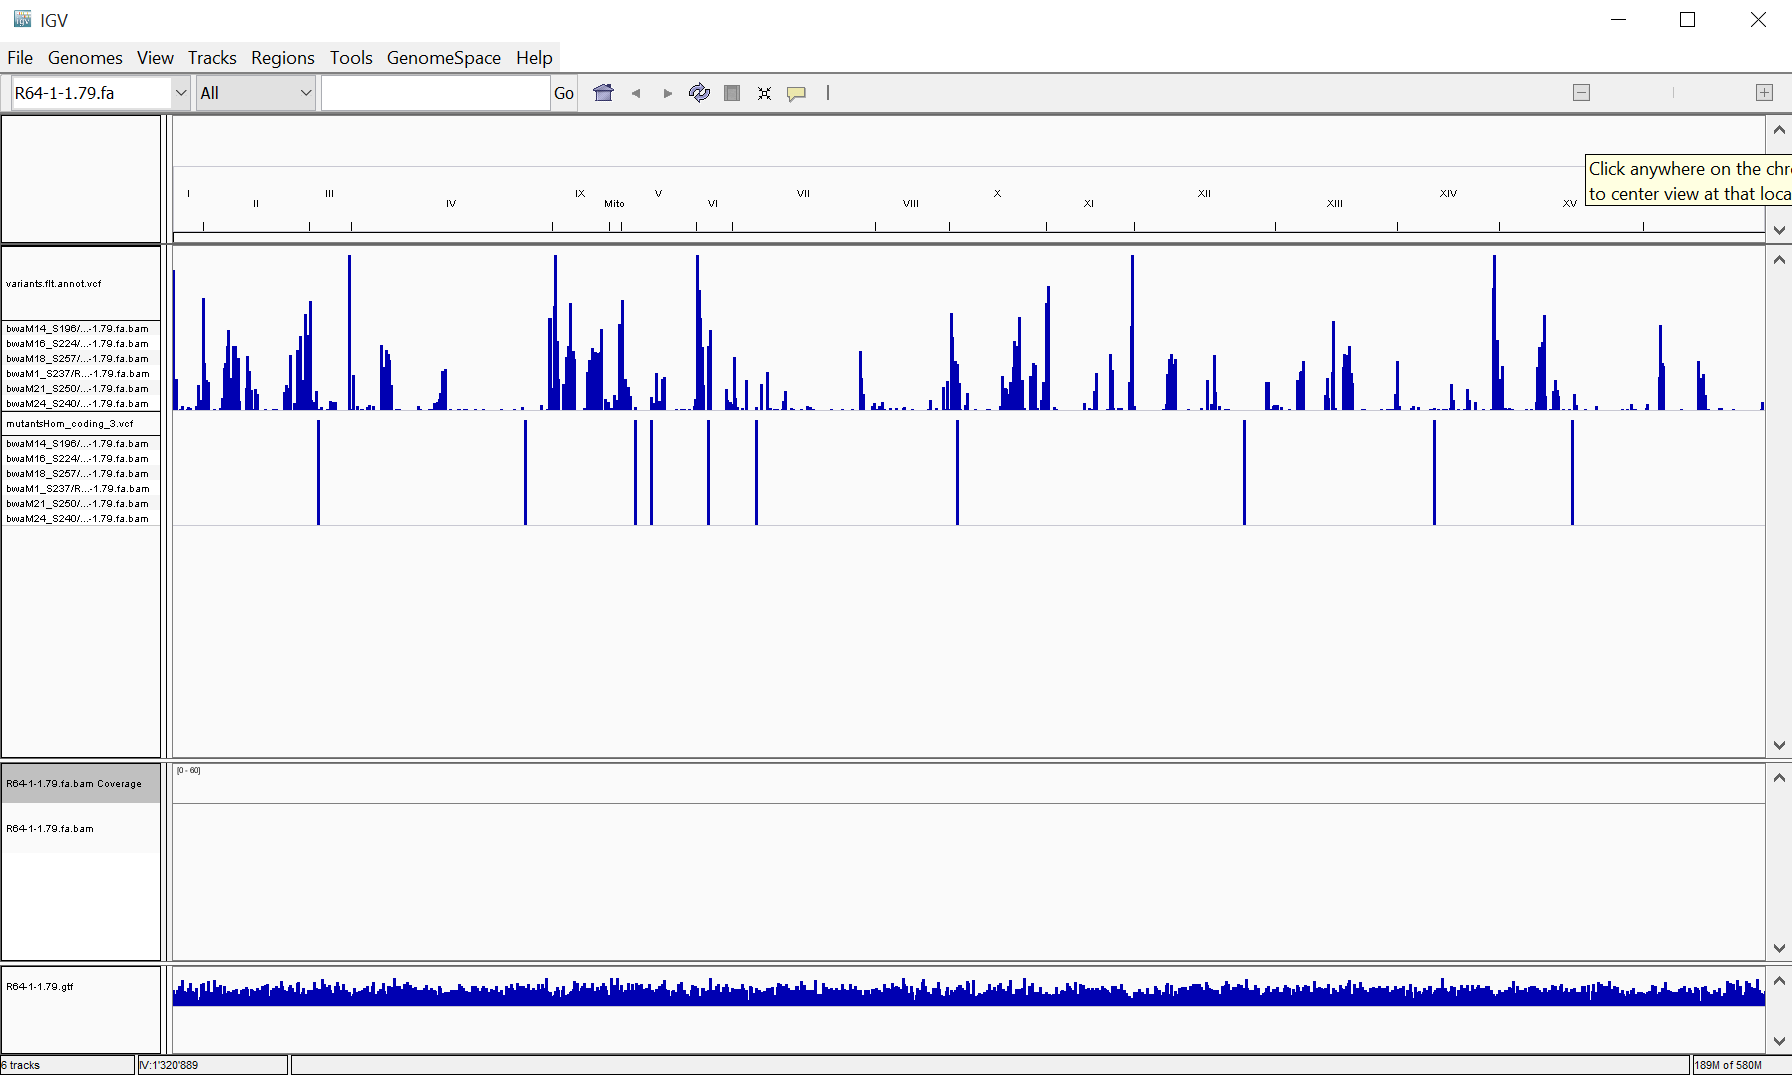
\includegraphics[width=\textwidth]{IGV_yeast}
\end{center}
\caption{SNP visualization using IGV}
\label{fig:yeastsnpigv}
\end{figure}


\end{description}

\section{Results}



We identified the following SNPs to be interesting. Table xy shows these observed mutations.

\begin{table}[]
\centering

\begin{tabular}{|l|l|l|}
\hline
 &  &  \\ \hline
 &  &  \\ \hline
 &  &  \\ \hline
\end{tabular}
\caption{SNPs}
\label{tab:yeastsnps}
\end{table}

\subsection{Mutant I}
Already known to be interferring w/ the TORC1 pathway. (Refernece)

\subsection{Mutant II}
Already known to be interferring w/ the TORC1 pathway. (Refernece)

\subsection{Mutant III}
Shows some significant differences. ...interesting.

\section{Analysis and Discussion}

\pagebreak
\part{Paracasei}
\setcounter{section}{0}

\section{Introduction}
(Very) Short introduction to cheese making. Collaboration w/ Agroscope. Sequencing of different starters that they have in their library.

What is the goal of our work?

Which genes are associated with the growth phenotype?

What is the biochemical relation between VSC and the growth phenotype?


\section{Data and Methods}
We had the data from ...?

We used the following Pipeline...

Although the overall quality of the data was acceptable, we used sickle to correct and filter...

\section{Results}




\section{Analysis and Discussion}

\pagebreak
\appendix
\section{Appendix Some picture of data processing pipeline}
\section{Appendix Second picture of data processing pipeline}

\printbibliography

\end{document}